\section{Ex2.5-----------------}\label{sec:Normal_Distribution}

\subsection{Testo esercizio}
La funzione $f(x;\mu;\sigma)$ nota come distribuzione normale o gaussiana è data come 
$$f(x,\mu,\sigma) = \frac{1}{{\sigma\sqrt{2\pi}}}
e^{{{-\left({x-\mu}\right)^2}\mathord{\left/{\vphantom{{-\left({x-\mu}\right)^2}{2\sigma^2}}}\right.\kern-\nulldelimiterspace}{2\sigma^2}}}$$
dove $\mu$ è la media e $\sigma$ è la deviazione standard.


\begin{itemize}
    \item[a)] Creare una funzione $normalDistribuition(x,mu,sigma)$ che restituisce il 
     valore di $f(x,\mu,\sigma)$.
    
    \item[b)] Usa questa funzione per tracciare la gaussiana per $-5<x<5$ con $\mu=0$ e 
    $\sigma=1$.
    
    \item[c)] Usa questa funzione per tracciare le gaussiane per $-5<x<5$ con $\mu=0$ e 
    $\sigma=2$ e $0.5$ nelle stesso diagramma.
    
    \item[d)] Usa questa funzione per tracciare le gaussiane per $-5<x<5$ con $\sigma=1$ 
    e $\mu=0$, $1$, $2$ in 3 diagrammi nelle stessa figura.
\end{itemize}

\subsection{Descrizione}

\subsection{Codice esercizio}
%\begin{minipage}{\linewidth}
\lstinputlisting[caption = {Funzione normalDistribuition}]
{cap/cap2/src/function/normalDistribuition.m}



%\end{minipage}
\pagebreak
\subsection{Risultato}

\lstinputlisting[caption = {Script Ex2.05-b}]{cap/cap2/src/script/script205b.m}
\begin{figure}[h]
    \centering
  %  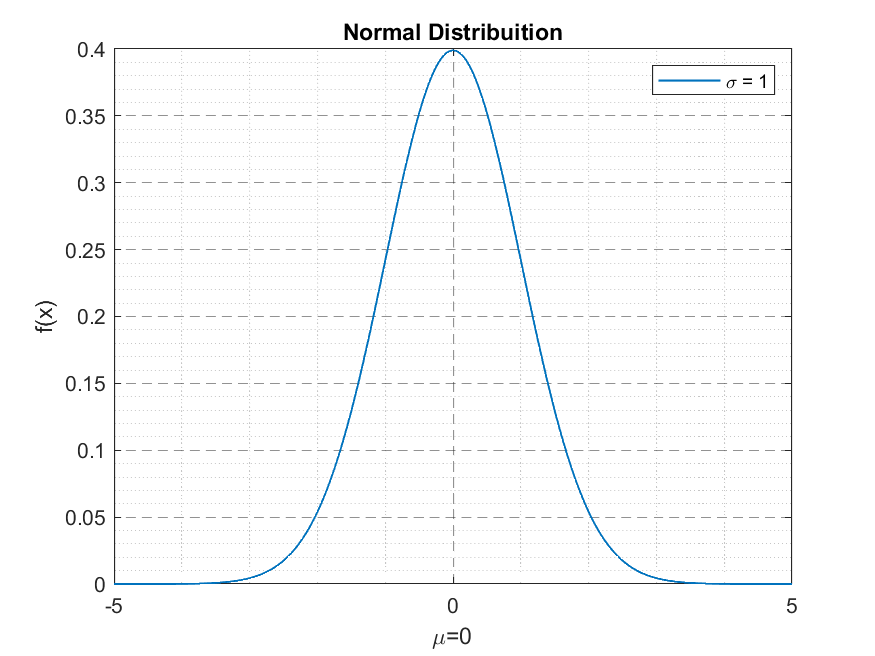
\includegraphics[width=1\linewidth]{diagram/script205b}
    \label{fig:script205b}
\end{figure}

\lstinputlisting[caption = {Script Ex2.05-c}]{cap/cap2/src/script/script205c.m}
\begin{figure}[h]
    \centering
   % 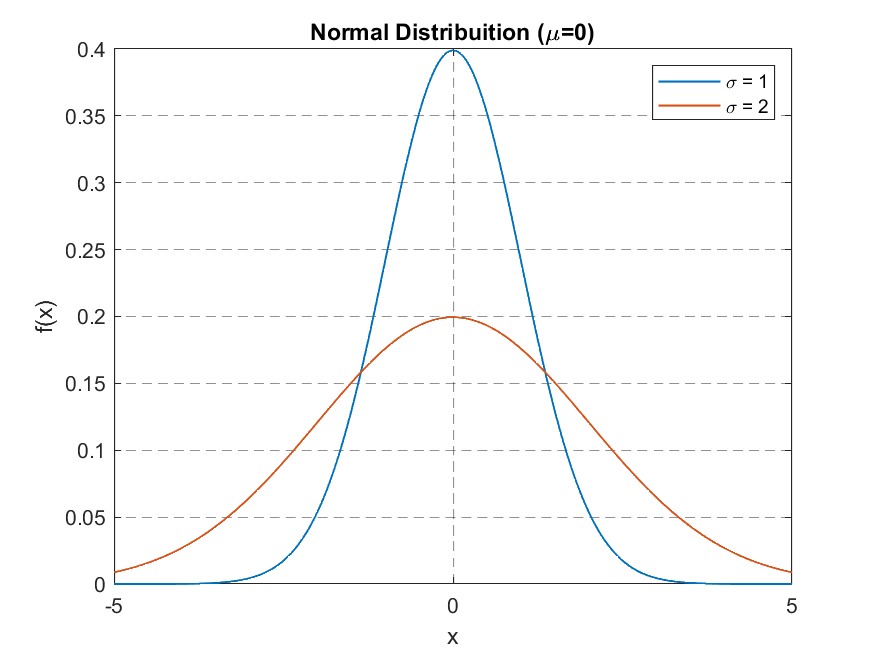
\includegraphics[width=1\linewidth]{cap/cap2/src/script205c}
    \label{fig:cript205c}
\end{figure}

\lstinputlisting[title = {Script Ex2.05-d}]
{cap/cap2/src/script/script205d.m}
\begin{figure}[h]
    \centering
    %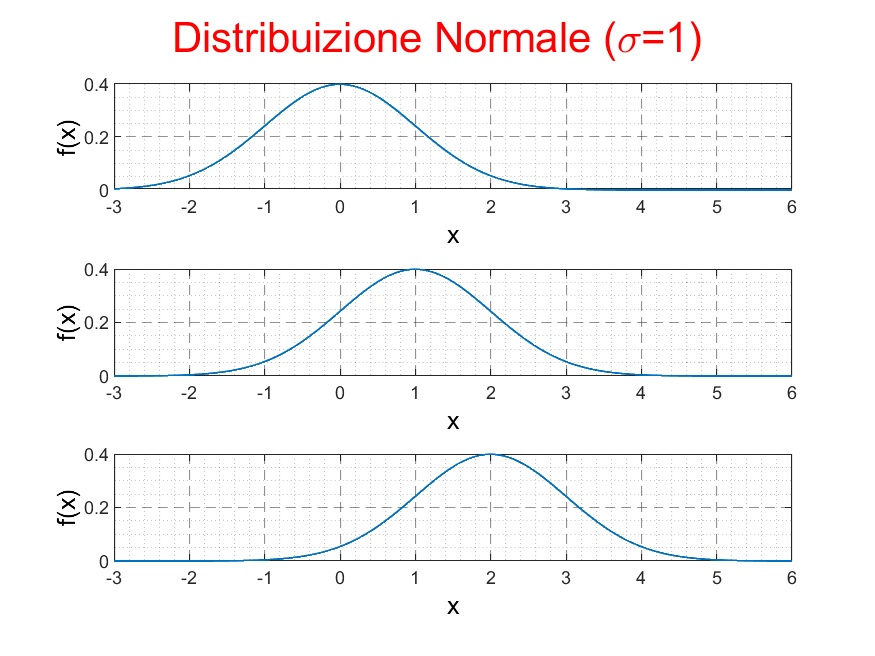
\includegraphics[width=0.95\linewidth]{diagram/script205d}
    \label{fig:cript205d}
\end{figure}